\documentclass[11pt]{article}

\usepackage[margin=1in]{geometry}
\usepackage{newtxtext,newtxmath}
\usepackage{amsmath,amssymb}
\usepackage{graphicx}
\usepackage{booktabs}
\usepackage[numbers,sort&compress]{natbib}
\usepackage{setspace}
\usepackage{lineno}
\usepackage{caption}
\usepackage{subcaption}
\usepackage{float}
\usepackage{placeins}
\usepackage{hyperref}

\onehalfspacing
\linenumbers
\graphicspath{{figures/}}

\title{Evaluation choices change infrared-versus-tabular rapid-intensification conclusions on {TC PRIMED}}

\author{
Muhammad Ahmad Amin \\
National University of Sciences and Technology (NUST), Islamabad, Pakistan \\
mamin.bscs24seecs@seecs.edu.pk
}

\date{}

\begin{document}
\maketitle

\begin{abstract}
Deep-learning studies sometimes conclude that storm-centered infrared (IR) imagery improves probabilistic tropical cyclone (TC) rapid intensification (RI) forecasts relative to scalar predictors. On public NOAA {TC PRIMED} (AL+EP; train/validation 2017--2022; test 2023--2024; 75 storms, 393 RI events), we compare a tabular multilayer perceptron (MLP), an IR convolutional network, gated fusion, and gradient-boosting machines (GBMs) for 24\,h RI ($\geq 30$\,kt).

Three results follow. First, the neural-versus-GBM ranking depends on the classical-control protocol: a small validation grid selects sklearn-default-like settings (three-seed isotonic Brier skill score, BSS, $+0.11$), whereas a post-hoc regularized GBM (\texttt{subsample}=$0.8$, \texttt{max\_features}=\texttt{sqrt}) reaches $+0.21$ on the test set yet is worse on validation Brier; the latter figure is therefore not a validation-locked baseline. Second, positive-class weighting produces a large raw MLP deficit relative to other weighted pathways (BSS $-0.43$ versus imagery near zero and fusion $-0.13$); isotonic recalibration largely closes BSS gaps and unweighted training restores tabular skill, but weighting still changes imagery ROC-AUC ($0.74$ versus $0.78$). Third, under matched unweighted training with shared trainer defaults, fusion does not significantly exceed the MLP (isotonic $\Delta$BSS $+0.03$ $[-0.01,0.07]$), and imagery does not significantly exceed an MLP trained on six IR scalars alone (scalars-only minus imagery $+0.05$ $[-0.01,0.10]$; AUC $0.84$ versus $0.78$).

Unweighted neural controls and the regularized GBM sensitivity were introduced after inspection of the weighted runs. The study assesses evaluation design on {TC PRIMED} and is complementary to the SHIPS/IR ablation of \citet{lagerquist2025}.
\end{abstract}

\section{Introduction}
\label{sec:intro}

Rapid intensification (RI; $\geq 30$\,kt in 24\,h) remains difficult to predict \citep{kaplan2003,kaplan2010,kaplan2015}. Operational statistical guidance based on the Statistical Hurricane Intensity Prediction Scheme (SHIPS) remains central to RI forecasting \citep{kaplan2015,demaria2021}. Convolutional neural networks (CNNs) applied to storm-centered IR imagery have reported skill relative to selected baselines \citep{griffin2022}.

\citet{lagerquist2025} address the closest physical and data-source question: on SHIPS developmental scalars plus CIRA IR fields, with operational baselines and explainable AI, SHIPS predictors dominate and full IR fields contribute only a modest incremental gain. The present study asks a complementary evaluation question on the public NOAA {TC PRIMED} archive. Specifically, we examine whether class weighting, unmatched probability calibrators, storm-ignorant uncertainty quantification, and post-hoc classical hyperparameters can alter pathway rankings in an otherwise similar IR-versus-tabular comparison. The analysis isolates four design choices: (i)~class weighting with and without recalibration, (ii)~matched calibrators across models, (iii)~storm-clustered uncertainty on seed-averaged predictions, and (iv)~validation-locked versus post-hoc GBM hyperparameters.

The contributions are as follows. We document a class-weighting artifact in which the weighted raw MLP appears much weaker than weighted imagery and fusion under the same loss. We introduce unweighted neural controls and show that weighting also changes imagery discrimination, not only calibration. We adopt a validation-selected default GBM as the primary classical control and report a labeled post-hoc regularized GBM sensitivity to demonstrate protocol dependence of the neural-versus-GBM comparison. Primary neural-versus-GBM inference uses seed-averaged paired contrasts, with single-seed member comparisons as a secondary fairness check. Informative IR comparisons under matched inputs include fusion versus the tabular MLP and an IR-scalars-only MLP versus imagery. Supporting analyses include a matched feature ladder, rate-matched detection diagnostics, a validation-chosen MLP operating point, and sample-versus-clustered and by-year uncertainty checks.

The scope is restricted to evaluation design on public {TC PRIMED}. We do not include matched operational SHIPS-RII or DTOPS baselines \citep{demaria2021,onderlinde2018} and do not attempt explainable-AI attribution.

\citet{lagerquist2025} provide the closest published IR-versus-scalar RI ablation, using SHIPS predictors, CIRA IR, operational baselines, and explainable AI. \citet{griffin2022} emphasize operational comparison of CNN guidance. Image-centric RI benchmarks explore spatial predictors with comparatively less emphasis on strong classical tabular controls \citep{bai2020}. The present work complements that literature by stress-testing loss weighting, calibrator matching, storm clustering, and classical-control provenance on a fully public data stack.

Verification follows the Brier score and Brier skill score (BSS) relative to climatology \citep{brier1950,hsu1986,wilks2011}. Proper scoring rules reward calibrated probabilistic forecasts \citep{gneiting2007}. Murphy's decomposition separates reliability and resolution \citep{murphy1973}. Temperature scaling and isotonic regression are widely used probability calibrators \citep{guo2017,niculescu2005}; \citet{lagerquist2025} likewise apply isotonic calibration to neural-network probabilities. Broader atmospheric machine-learning guidance emphasizes trustworthy evaluation and baseline strength \citep{mcgovern2019,mcgovern2019b,ebertuphoff2021,chase2022}. Strong classical and neural baselines remain central in related forecasting applications \citep{gagne2019,rasp2020}.

\section{Results}
\label{sec:results}

Unless noted otherwise, intervals are storm-clustered $95\%$ intervals on the 75 test storms. Contrasts are not multiplicity-corrected. Category~1--2 subset results are exploratory. Primary neural-versus-GBM and pathway comparisons follow the seed-averaged paired contrasts in Table~\ref{tab:paired}; single-seed rows in Table~\ref{tab:singleseed} provide a secondary fairness check on matched seed pairs. Data, models, and verification procedures are described in Materials and Methods.

\subsection{Overall skill}

Table~\ref{tab:main} reports seed-averaged test BSS. Under class weighting, the raw MLP BSS of $-0.43$ contrasts with weighted raw imagery near zero and weighted raw fusion of $-0.13$; isotonic recalibration recovers skill for all three pathways. Unweighted training is the primary neural protocol. The primary GBM is the validation-grid winner at the sklearn-default corner, reported as a three-seed average; the deterministic default row is nearly identical. The regularized GBM row is the post-hoc sensitivity described in Materials and Methods.

\begin{table}[H]
\centering
\caption{Seed-averaged overall test BSS with storm-clustered 95\% intervals. Test set: 75 storms, 393 RI events. Primary neural protocol is unweighted; primary GBM is validation-selected defaults.}
\label{tab:main}
\begin{tabular}{llcc}
\toprule
Model & Calibrator / protocol & BSS [CI] & $\bar p$ \\
\midrule
MLP weighted & raw & $-0.43$ $[-1.09,-0.03]$ & $0.131$ \\
MLP weighted & isotonic & $+0.20$ $[0.10,0.27]$ & $0.052$ \\
Imagery weighted & raw & $+0.00$ $[-0.09,0.10]$ & $0.030$ \\
Imagery weighted & isotonic & $+0.05$ $[0.02,0.09]$ & $0.045$ \\
Fusion weighted & raw & $-0.13$ $[-0.66,0.16]$ & $0.110$ \\
Fusion weighted & isotonic & $+0.21$ $[0.11,0.27]$ & $0.050$ \\
\midrule
MLP unweighted & raw & $+0.20$ $[0.07,0.29]$ & $0.058$ \\
MLP unweighted & isotonic & $+0.20$ $[0.09,0.27]$ & $0.053$ \\
Imagery unweighted & raw & $+0.03$ $[-0.01,0.07]$ & $0.031$ \\
Imagery unweighted & isotonic & $+0.03$ $[-0.02,0.07]$ & $0.046$ \\
Fusion unweighted & raw & $+0.24$ $[0.11,0.33]$ & $0.046$ \\
Fusion unweighted & isotonic & $+0.22$ $[0.12,0.30]$ & $0.050$ \\
IR-scalars-only MLP & isotonic & $+0.08$ $[0.03,0.11]$ & $0.047$ \\
\midrule
GBM default 3-seed avg (primary) & isotonic & $+0.11$ $[-0.05,0.21]$ & $0.065$ \\
GBM default 3-seed avg & raw & $+0.13$ $[-0.06,0.24]$ & $0.055$ \\
GBM default 3-seed avg & Platt & $+0.10$ $[-0.04,0.20]$ & $0.059$ \\
GBM deterministic default & isotonic & $+0.11$ $[-0.05,0.22]$ & $0.064$ \\
GBM regularized (post hoc) & isotonic & $+0.21$ $[0.11,0.27]$ & $0.058$ \\
\bottomrule
\end{tabular}
\end{table}

Weighted isotonic MLP skill matches the unweighted MLP, but weighted imagery ROC-AUC is $0.74$ compared with $0.78$ under unweighted training, indicating that class weighting alters the learned ranking rather than only the probability scale. The post-hoc regularized GBM attains seed-averaged neural BSS ($+0.21$) while losing the validation grid. Because that configuration was selected after inspection of test outcomes, the $+0.21$ figure is not presented as a locked baseline; the substantive conclusion is that the neural-versus-GBM ranking is sensitive to the classical-control protocol.

\subsection{Paired seed-averaged contrasts}

Table~\ref{tab:paired} summarizes the primary paired inference. The fusion-minus-MLP contrast remains inconclusive under storm clustering (interval includes zero). Imagery versus the full tabular MLP is negative overall, but the comparison confounds inputs: the MLP receives environmental predictors plus IR scalars, whereas the imagery network receives only the image. The matched IR-content comparison is therefore IR-scalars-only MLP versus imagery. The paired $\Delta$BSS of $+0.05$ $[-0.01,0.10]$ includes zero and does not establish equivalence; nonetheless, the scalars-only model has higher ROC-AUC ($0.841$ versus $0.778$) and is the only one of the two whose absolute BSS interval excludes zero ($+0.08$ $[0.03,0.11]$ versus imagery $+0.03$ $[-0.02,0.07]$). Under the shared trainer, imagery is not shown to provide more usable information than six IR scalars, despite roughly $13\times$ more parameters in the imagery CNN. Fusion's still larger capacity likewise does not yield a statistically supported gain over the tabular MLP. The Category~1--2 imagery-minus-MLP contrast reaches an uncorrected $95\%$ lower edge at $-0.00$ over 32 storms and is treated as exploratory.

Neural pathway comparisons use shared trainer defaults without architecture search. Statements that fusion does not significantly exceed the MLP therefore refer to this protocol, not to a searched upper bound on fusion skill.

\begin{table}[H]
\centering
\caption{Seed-averaged paired $\Delta$BSS with storm-clustered 95\% intervals. Matched calibrators only.}
\label{tab:paired}
\begin{tabular}{llcc}
\toprule
Contrast & Scope & $\Delta$BSS & CI \\
\midrule
Fusion iso.\ $-$ MLP iso. & overall & $+0.03$ & $[-0.01,0.07]$ \\
IR-scalars MLP iso.\ $-$ imagery iso. & overall & $+0.05$ & $[-0.01,0.10]$ \\
Fusion iso.\ $-$ GBM default iso. & overall & $+0.11$ & $[0.04,0.23]$ \\
MLP iso.\ $-$ GBM default iso. & overall & $+0.09$ & $[0.01,0.20]$ \\
Fusion iso.\ $-$ GBM reg.\ (post hoc) & overall & $+0.02$ & $[-0.02,0.06]$ \\
MLP iso.\ $-$ GBM reg.\ (post hoc) & overall & $-0.01$ & $[-0.06,0.05]$ \\
Imagery iso.\ $-$ MLP iso. & overall & $-0.16$ & $[-0.24,-0.07]$ \\
Imagery iso.\ $-$ MLP iso. & Cat.~1--2 & $-0.20$ & $[-0.32,-0.00]$ \\
\bottomrule
\end{tabular}
\end{table}

\subsection{Single-seed contrasts}

Table~\ref{tab:singleseed} pairs each neural seed with the GBM member trained under the same seed. Because every seed evaluates the same 75 storms, these rows are not independent replications of the test set. Relative to validation-selected default members, two intervals exclude zero (seed~44), one sits at the boundary (seed~43 fusion, lower edge $0.00$), and the remainder include zero; the median $\Delta$BSS across the three fusion (MLP) seeds is $+0.08$ ($+0.08$). Relative to post-hoc regularized members, all six intervals include zero, with median $\Delta$BSS near zero.

\begin{table}[H]
\centering
\caption{Single-seed neural isotonic versus same-seed GBM member isotonic (storm-clustered 95\% intervals). Secondary fairness check on matched seed pairs; identical test storms in every seed.}
\label{tab:singleseed}
\begin{tabular}{llcc}
\toprule
Seed & Contrast & $\Delta$BSS & CI \\
\midrule
\multicolumn{4}{l}{\emph{Versus default GBM member (validation-selected HP)}} \\
42 & Fusion $-$ GBM & $+0.08$ & $[-0.00,0.18]$ \\
42 & MLP $-$ GBM & $+0.07$ & $[-0.01,0.17]$ \\
43 & Fusion $-$ GBM & $+0.08$ & $[0.00,0.21]$ \\
43 & MLP $-$ GBM & $+0.08$ & $[-0.00,0.18]$ \\
44 & Fusion $-$ GBM & $+0.11$ & $[0.04,0.21]$ \\
44 & MLP $-$ GBM & $+0.09$ & $[0.01,0.20]$ \\
\midrule
\multicolumn{4}{l}{\emph{Versus regularized GBM member (post hoc HP)}} \\
42 & Fusion $-$ GBM & $-0.01$ & $[-0.06,0.05]$ \\
42 & MLP $-$ GBM & $-0.01$ & $[-0.06,0.05]$ \\
43 & Fusion $-$ GBM & $-0.01$ & $[-0.05,0.06]$ \\
43 & MLP $-$ GBM & $-0.01$ & $[-0.07,0.05]$ \\
44 & Fusion $-$ GBM & $+0.02$ & $[-0.03,0.08]$ \\
44 & MLP $-$ GBM & $+0.00$ & $[-0.06,0.07]$ \\
\bottomrule
\end{tabular}
\end{table}

\subsection{Tabular feature ladder}

Table~\ref{tab:ladder} reports matched isotonic BSS by feature set. The full tabular MLP rung is the same unweighted MLP isotonic series as in Table~\ref{tab:main}. The GBM column uses the validation-selected default three-seed average. The paired environment-to-full MLP contrast is $+0.05$ $[-0.01,0.09]$ and does not exclude zero under clustering. Fusion minus that same MLP is $+0.03$ $[-0.01,0.07]$, consistent with Table~\ref{tab:paired}.

\begin{table}[H]
\centering
\caption{Feature ladder with matched isotonic calibrators and storm-clustered 95\% BSS intervals. Full MLP matches Table~\ref{tab:main} unweighted MLP isotonic. GBM is the default three-seed average.}
\label{tab:ladder}
\begin{tabular}{lcc}
\toprule
Feature set & GBM default iso.\ [CI] & MLP / fusion iso.\ [CI] \\
\midrule
Environment only (8) & $+0.10$ $[-0.12,0.20]$ & $+0.16$ $[0.06,0.23]$ \\
Environment $+$ IR scalars (14) & $+0.11$ $[-0.05,0.21]$ & $+0.20$ $[0.09,0.27]$ \\
IR scalars only (6) & -- & $+0.08$ $[0.03,0.11]$ \\
$+$ image (fusion iso.) & -- & $+0.22$ $[0.12,0.30]$ \\
Imagery only (CNN) & -- & $+0.03$ $[-0.02,0.07]$ \\
\bottomrule
\end{tabular}
\end{table}

\subsection{Discrimination and detection}

Seed-averaged ROC-AUC values are $0.905$ (unweighted MLP), $0.904$ (fusion), $0.778$ (imagery), $0.841$ (IR-scalars-only MLP), $0.889$ (default GBM), and $0.906$ (post-hoc regularized GBM). Weighted imagery AUC is $0.74$. Mean per-seed neural AUCs are slightly lower than AUCs computed on seed-averaged probabilities; the two summaries are not interchangeable.

Table~\ref{tab:detection} reports diagnostic detection skill at an alert rate equal to the test RI rate. Fusion attains the highest CSI point estimate, but intervals overlap those of the MLP and GBMs. At fixed alert rate the score is rank-based, so one raw row is shown per model. Default GBM metrics are recomputed on the primary three-seed-average raw probabilities and coincide with the deterministic seed-42 row at reported precision (score-vector correlation $>0.999$ under sklearn defaults). A validation CSI-maximizing threshold for the unweighted MLP yields CSI $0.25$ at threshold $0.20$, close to the diagnostic row.

\begin{table}[H]
\centering
\caption{Diagnostic detection at alert rate equal to the test RI rate on seed-averaged raw scores (storm-clustered 95\% intervals). This operating point uses the test base rate and is not a deployable threshold. GBM default uses the primary three-seed average.}
\label{tab:detection}
\scriptsize
\begin{tabular}{lcccc}
\toprule
Model & Thr. & CSI [CI] & FAR [CI] & POD [CI] \\
\midrule
MLP & $0.29$ & $0.25$ $[0.16,0.34]$ & $0.60$ $[0.45,0.75]$ & $0.40$ $[0.29,0.52]$ \\
Fusion & $0.27$ & $0.28$ $[0.18,0.37]$ & $0.56$ $[0.43,0.72]$ & $0.44$ $[0.32,0.55]$ \\
GBM default (3-seed) & $0.30$ & $0.24$ $[0.16,0.31]$ & $0.61$ $[0.49,0.74]$ & $0.39$ $[0.29,0.49]$ \\
GBM reg.\ (post hoc) & $0.25$ & $0.27$ $[0.18,0.36]$ & $0.57$ $[0.46,0.72]$ & $0.43$ $[0.30,0.55]$ \\
Imagery & $0.12$ & $0.10$ $[0.05,0.15]$ & $0.82$ $[0.71,0.91]$ & $0.18$ $[0.10,0.26]$ \\
\bottomrule
\end{tabular}
\end{table}

\subsection{Uncertainty design checks}

\begin{table}[H]
\centering
\caption{Sample bootstrap versus storm-clustered 95\% BSS intervals for unweighted MLP raw (seed-averaged). Point BSS $=+0.20$.}
\label{tab:sample}
\begin{tabular}{lcc}
\toprule
Resampling & BSS lo & BSS hi \\
\midrule
IID sample bootstrap & $0.17$ & $0.23$ \\
Storm-clustered bootstrap & $0.07$ & $0.29$ \\
\bottomrule
\end{tabular}
\end{table}

\begin{table}[H]
\centering
\caption{Test-set composition and seed-averaged isotonic BSS by season (point estimates only; within-year intervals are wide). Imagery remains below IR-scalars-only in both years.}
\label{tab:year}
\begin{tabular}{lcccccccc}
\toprule
Season & $n$ & RI & Rate & MLP & Fusion & IR scalars & Imagery \\
\midrule
2023 & 4953 & 223 & $4.5\%$ & $+0.24$ & $+0.26$ & $+0.09$ & $+0.05$ \\
2024 & 3160 & 170 & $5.4\%$ & $+0.14$ & $+0.18$ & $+0.07$ & $+0.01$ \\
\bottomrule
\end{tabular}
\end{table}

Fusion exceeds the MLP in by-year point estimates in both seasons ($+0.26$ versus $+0.24$ in 2023; $+0.18$ versus $+0.14$ in 2024), while the pooled fusion-minus-MLP contrast still includes zero ($+0.03$ $[-0.01,0.07]$). Within-year storm counts are smaller and intervals are wider; the pooled clustered contrast remains the primary summary. The consistent sign of the by-year gaps is a directional lean in the point estimates only and does not by itself establish a fusion advantage.

\subsection{Reliability}

Figure~\ref{fig:reliability} shows reliability diagrams for the unweighted MLP and fusion pathways (raw and isotonic) for seed~42.

\begin{figure}[H]
\centering
\begin{subfigure}{0.48\linewidth}
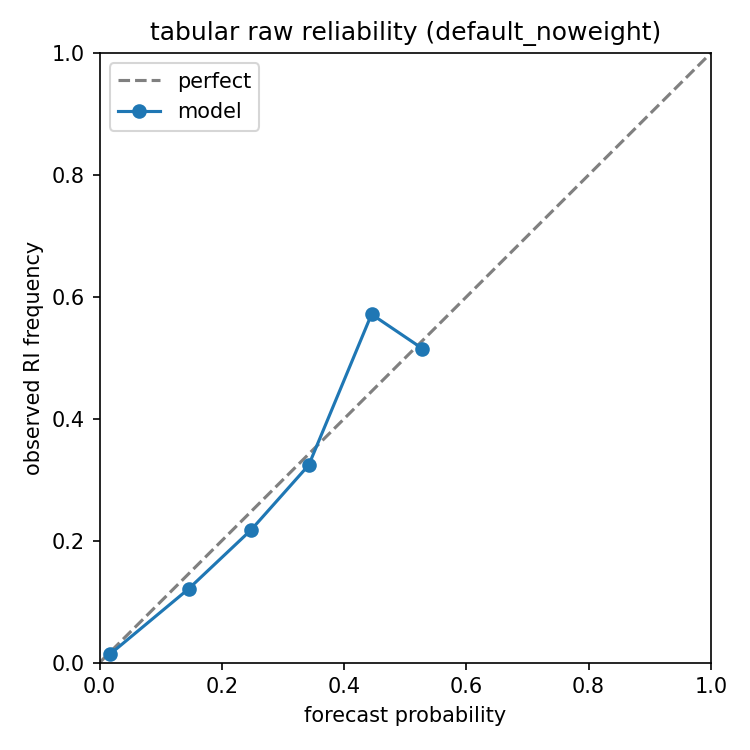
\includegraphics[width=\linewidth]{reliability_mlp_noweight_raw.png}
\caption{MLP unweighted (raw)}
\end{subfigure}\hfill
\begin{subfigure}{0.48\linewidth}
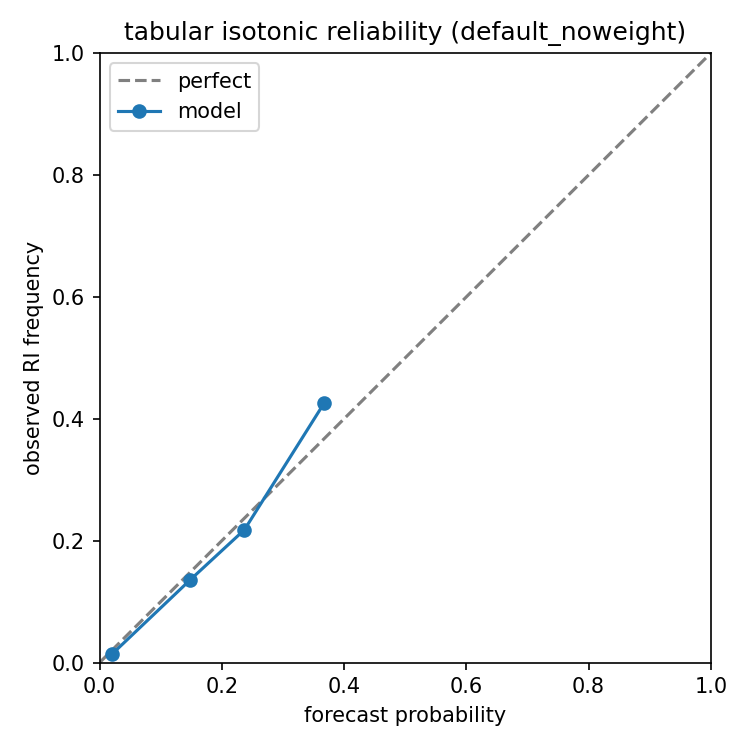
\includegraphics[width=\linewidth]{reliability_mlp_noweight_iso.png}
\caption{MLP unweighted (isotonic)}
\end{subfigure}

\vspace{0.6em}

\begin{subfigure}{0.48\linewidth}
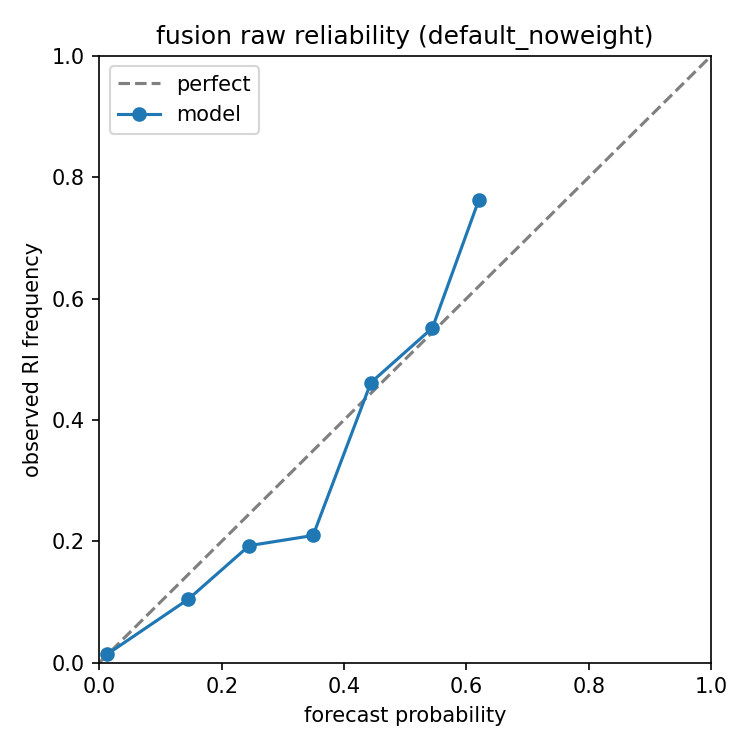
\includegraphics[width=\linewidth]{reliability_fusion_noweight_raw.png}
\caption{Fusion unweighted (raw)}
\end{subfigure}\hfill
\begin{subfigure}{0.48\linewidth}
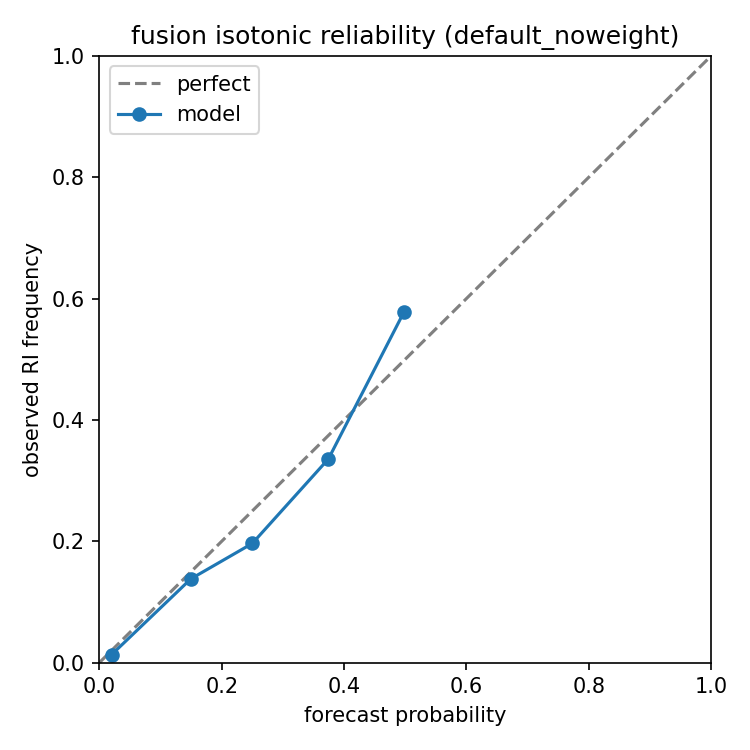
\includegraphics[width=\linewidth]{reliability_fusion_noweight_iso.png}
\caption{Fusion unweighted (isotonic)}
\end{subfigure}
\caption{Reliability diagrams (seed 42, unweighted primary runs). Mean predicted probability is near the test RI rate ($\approx 0.048$).}
\label{fig:reliability}
\end{figure}
\FloatBarrier

\section{Discussion}
\label{sec:discussion}

Taken together, the results show that several evaluation choices materially affect IR-versus-tabular RI rankings on {TC PRIMED}. The validation-selected default-like GBM (BSS approximately $+0.11$) is the primary classical baseline. A single post-hoc regularized configuration reaches $+0.21$ and can match seed-averaged neural skill, but because it was identified after inspection of test outcomes it is not a locked baseline. The supported claim is protocol dependence of the neural-versus-GBM comparison, not a demonstrated validation-locked benefit of that regularized setting.

Class weighting produces a large raw MLP deficit alongside near-zero weighted imagery skill and weak weighted fusion skill until isotonic recalibration. Isotonic adjustment removes much of the BSS gap, yet imagery AUC still changes under weighting, indicating that representations as well as probability scales are affected. Under shared trainer defaults, fusion does not significantly exceed the MLP in the pooled contrast, even though by-year point estimates lean slightly toward fusion. The negative imagery-versus-full-MLP contrast is expected given unequal inputs; the matched IR comparison is IR-scalars-only versus imagery, where imagery is not shown to carry more usable information than six scalars despite substantially higher capacity. Fusion's additional capacity likewise yields no demonstrated pooled gain over the tabular MLP under the same protocol. Relative to the validation-selected GBM, seed-averaged neural models remain ahead in point BSS; that lead should not be conflated with comparisons against the post-hoc regularized GBM.

\subsection{Limitations}

The study has several limitations. First, it does not include matched SHIPS-RII or DTOPS baselines. Second, skill is assessed on a single two-season holdout; within-year intervals in Table~\ref{tab:year} are wide. Third, neural hyperparameters are not tuned beyond shared trainer defaults, whereas the GBM receives a small validation grid; neural scores are therefore protocol lower bounds rather than architecture ceilings, and fusion-versus-MLP conclusions concern evaluation design under one trainer. Fourth, imagery and fusion have roughly an order of magnitude more parameters than the MLP, and imagery uses single-frame IRWIN only; the capacity gap strengthens the scalars-versus-imagery reading when imagery still fails to outperform scalars, but also means that untuned fusion is not a search over fusion architectures. Fifth, the Category~1--2 subset is exploratory (32 storms), and the imagery-minus-MLP edge there is borderline at an uncorrected $95\%$ level. Sixth, unweighted controls and the regularized GBM sensitivity were chosen after inspection of weighted results. Seventh, multiple contrasts are reported without multiplicity correction, and rate-matched detection uses the test base rate as a diagnostic only.

\subsection{Conclusions}

On public {TC PRIMED}, evaluation design choices change conclusions about IR-versus-tabular 24\,h RI skill. The validation-selected default-like GBM (BSS $+0.11$) is the primary classical baseline; a post-hoc regularized configuration that reaches $+0.21$ is optimistic relative to the locked protocol. Class weighting produces a pronounced raw MLP deficit relative to weighted imagery and fusion; isotonic recalibration and unweighted training remove most of the BSS gap, but weighting still shifts imagery discrimination. Under shared trainer defaults, fusion does not significantly exceed the unweighted MLP, and imagery does not significantly exceed an IR-scalars-only MLP despite much higher capacity. Against validation-selected default GBMs, seed-averaged neural models lead in point BSS (MLP/fusion $\Delta$ approximately $+0.09$ to $+0.11$), with clustered intervals that mostly exclude zero but remain wide; single-seed contrasts are weaker, and contrasts against the post-hoc regularized GBM are inconclusive. These findings motivate matching loss and calibrators across pathways, locking classical hyperparameters on validation, and clustering uncertainty by storm before attributing skill gains to imagery or fusion.

\section{Materials and Methods}
\label{sec:methods}

\subsection{Experimental and technical design}

The study compares four pathways for probabilistic 24\,h RI prediction on public {TC PRIMED}: a tabular MLP, an IR CNN, gated fusion of tabular and image encoders, and GBMs. Training seasons are 2017--2022 with a storm-wise validation holdout; testing uses 2023--2024. Primary neural training uses unweighted binary cross-entropy; class-weighted training is retained as an ablation. Classical controls are selected by a validation Brier grid, with a labeled post-hoc regularized GBM sensitivity. Inference averages three seeds and uses storm-clustered bootstraps. Pairwise claims use matched calibrators only.

\subsection{Data}

We use {TC PRIMED} IRWIN imagery and environmental diagnostics \citep{razin2023,tcprimed} for the Atlantic (AL) and eastern North Pacific (EP) basins (33\,878 samples; 1\,409 RI events). The RI label is a 24\,h intensity increase of at least $30$\,kt. Tabular inputs comprise 14 features: eight environmental and storm-state predictors (\texttt{sst\_c}, low- and high-level shear, potential intensity, precipitable water, distance to land, storm translation speed, and intensity) and six IR scalars (annulus standard deviations, eye maximum and mean brightness temperature, and cold-cloud fractions). Imagery pathways use a single-time IRWIN field at $128\times 128$ resolution. Fusion combines gated tabular and image encoders.

Training and validation use seasons 2017--2022; the held-out test set uses 2023--2024 ($n=8113$; 75 storms; 393 RI events; RI rate $4.8\%$). On the test set the RI rate is $3.1\%$ in AL ($n=4999$) and $7.6\%$ in EP ($n=3114$). Validation comprises a storm-wise $25\%$ holdout within the training seasons. All calibrators are fit on validation data only.

\subsection{Models and training}

Neural models are trained with AdamW, weight decay, and early stopping on validation Brier score, with restoration of the best checkpoint. Approximate parameter counts are $1.0\times 10^5$ for the MLP, $1.3\times 10^6$ for the imagery CNN, and $1.5\times 10^6$ for fusion. Neural hyperparameters are not tuned beyond a shared trainer configuration; pathway scores are therefore protocol-specific lower bounds rather than architecture ceilings. The GBM receives a small validation hyperparameter grid (described below). That asymmetry is intentional for assessing classical-control provenance and limits claims about neural performance under architecture search.

All neural pathways share the same trainer. The original runs minimize \texttt{BCEWithLogitsLoss} with positive-class weight $n_{\mathrm{neg}}/n_{\mathrm{pos}}$. The primary neural protocol uses unweighted binary cross-entropy; weighted runs are retained as a labeled ablation.

Models are trained with seeds 42, 43, and 44. Inferential claims average predicted probabilities across seeds and then apply one storm-clustered bootstrap per contrast. Because seeds share the same test storms, they are not independent replications of the test set.

\subsection{GBM protocols}

The primary classical control is selected from a validation grid that includes both default-like and regularized options: \texttt{subsample}$\in\{1.0,0.8,0.6\}$, \texttt{max\_features}$\in\{\mathrm{None},\texttt{sqrt}\}$, and \texttt{max\_depth}$\in\{\mathrm{None},3\}$. The configuration with the lowest mean raw validation Brier score is the sklearn-default corner (\texttt{subsample}=$1$, no feature subsampling, unlimited depth; validation Brier $0.04009$). Primary reporting uses the three-seed average of that setting. As a sensitivity analysis, the same three-seed average with \texttt{subsample}=$0.8$ and \texttt{max\_features}=\texttt{sqrt} yields a higher validation Brier ($0.04039$) but higher test BSS; we label this configuration the regularized GBM and do not treat it as validation-locked. A deterministic single-seed default GBM is reported for completeness. The primary calibrator is isotonic regression, selected by held-out half of validation Brier after fitting on the complementary half (isotonic $0.0392$, raw $0.0396$, Platt $0.0407$).

Unweighted neural retraining and the regularized GBM sensitivity were added after inspection of the weighted results and are disclosed as post-hoc analyses. Multiple pairwise contrasts are reported without multiplicity correction.

\subsection{Calibration and verification}

Pairwise model comparisons use matched calibrators only. BSS is computed relative to climatology with storm-clustered $95\%$ intervals over the 75 test storms. Discrimination is summarized by ROC-AUC on seed-averaged probabilities. Detection skill is assessed in two ways: (i)~an alert rate equal to the test RI rate, reported as a diagnostic ranking check that would not be available operationally without knowledge of the test base rate; and (ii)~a validation CSI-maximizing threshold for the unweighted MLP as a deployable operating-point check.

\section*{Data availability}
{TC PRIMED} data are available from NOAA/CIRA \citep{razin2023,tcprimed}. Code and metrics accompanying this study are available in the \texttt{hurricane-ri-forecast} repository.

\section*{Acknowledgments}
The author thanks NOAA/CIRA for public access to {TC PRIMED}.

\bibliographystyle{unsrtnat}
\bibliography{references}

\end{document}
